This chapter lists the requirements for an effect unit for a guitar. The requirements are based on the effect analysing and the Problem Statement.

\begin{figure}[htbp]
	\centering
\begin{picture}(0,0)%
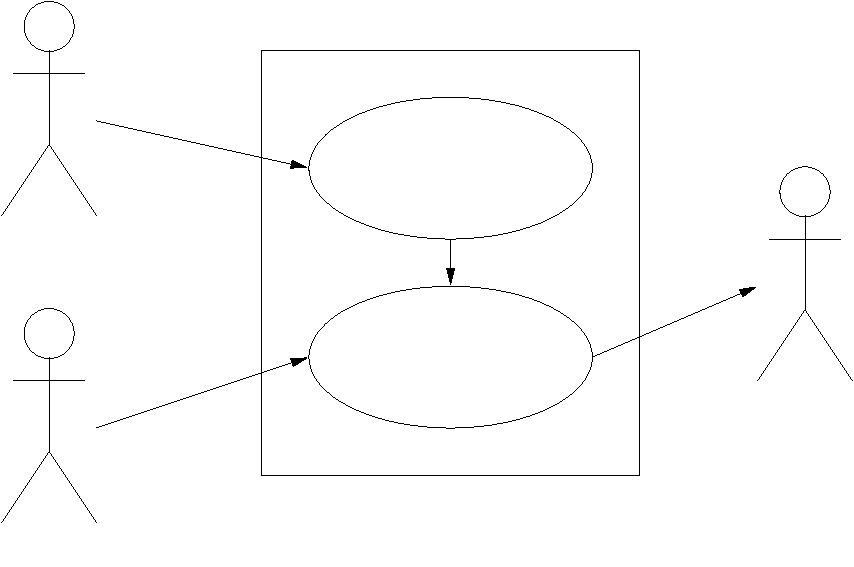
\includegraphics{Use_case.pdf}%
\end{picture}%
\setlength{\unitlength}{4144sp}%
%
\begingroup\makeatletter\ifx\SetFigFont\undefined%
\gdef\SetFigFont#1#2#3#4#5{%
  \reset@font\fontsize{#1}{#2pt}%
  \fontfamily{#3}\fontseries{#4}\fontshape{#5}%
  \selectfont}%
\fi\endgroup%
\begin{picture}(6507,4318)(1426,-4900)
\put(1531,-2491){User}%
\put(4546,-3346){Effect}%
\put(4276,-1906){Effect select}%
\put(7111,-3751){Amplifier}%
\put(1441,-4831){Guitar}%
\end{picture}%
	\caption{A graphically overview of wanted functionality in form of an use case digram.}
	\label{fig:use_case}
\end{figure}

